\subsubsection{Periods in the \Glsentrylong{pal} Structures}

First, we state that the function $t$ that translates 4-syllables from the halved archetypal model to the archetypal model preserves the period of the 4-syllable.
The function was defined in \Cref{sec:add.halved.tanslating}.

\begin{lemma}[$t$ Preserves Period]
	\label{lemma:t.preserves.period}
	The function $t$ preserves the period.
	\begin{align}
		|\sigma_1\sigma_2| = |t(\sigma_1\sigma_2)|
	\end{align}
\end{lemma}

\begin{proof}
	Let $\sigma_1\sigma_2 = \L^a\R^b\L^c\R^d$.
	\begin{align*}
		|\sigma_1\sigma_2| =  |\L^a\R^b\L^c\R^d|
		= a + b + c + d
		= |\A^a\B^b\C^c\D^d|
		= |t(\L^a\R^b\L^c\R^d)|
		= |t(\sigma_1\sigma_2)|
	\end{align*}
	\hfill $\blacksquare$
\end{proof}

\begin{theorem}[Periods Associated with Parameter Regions in the \gls{pal} Structures]
	\label{theorem:period.pal}
	\begin{enumerate}
		\item If a cycle in the halved archetypal model manifests as two coexisting cycles in the archetypal model, the period of either cycle is the same as the period of the cycle in the halved archetypal model.
		      \begin{align}
			      |T(\sigma)| = |T(s_2(\sigma))| = |\sigma|
		      \end{align}
		\item If a cycle in the halved archetypal model manifests as a single cycle in the archetypal model, the period of this cycle is double the period of the cycle in the halved archetypal model.
		      \begin{align}
			      |T(\sigma)| = 2 |\sigma|
		      \end{align}
	\end{enumerate}
\end{theorem}

\begin{proof} \phantom{x}
	\begin{enumerate}
		\item We know from \Cref{theorem:coexistence.even} that if the cycle $\sigma$ in the halved archetypal model manifests as two coexisting cycles in the archetypal model, $\sigma$ has an even number of rotations $n$.
		      And its translation is $T(\sigma) = t(\sigma_1\sigma_2) t(\sigma_3\sigma_4) \dots t(\sigma_{n-1}\sigma_n)$.
		      Combining this with the fact that $t$ preserves the period of its input as described in \Cref{lemma:t.preserves.period}, we can calculate the period of $T(\sigma)$ in the following way.
		      \begin{align*}
			      |T(\sigma)| & = |t(\sigma_1\sigma_2) t(\sigma_3\sigma_4) \dots t(\sigma_{n-1}\sigma_n)|           \\
			                  & = |t(\sigma_1\sigma_2)| + |t(\sigma_3\sigma_4)| + \dots + |t(\sigma_{n-1}\sigma_n)| \\
			                  & = |\sigma_1\sigma_2| + |\sigma_3\sigma_4| + \dots + |\sigma_{n-1}\sigma_n|          \\
			                  & = |\sigma_1\sigma_2 \dots \sigma_n| = |\sigma|
		      \end{align*}
		      So the period of the cycle $T(\sigma)$ in the archetypal model is the same as the period of the cycle $\sigma$ in the halved archetypal model.
		      The same calculation can be done for $T(s(\sigma))$ and is omitted here.
		\item Similarly, we know that if the cycle $\sigma$ in the halved archetypal model manifests as a single cycle in the archetypal model, $\sigma$ has an odd number of rotations $n$.
		      And its translation is $T(\sigma) = t(\sigma_1\sigma_2) \dots t(\sigma_n\sigma_1) \dots t(\sigma_{n-1}\sigma_n)$.
		      Its period can be calculated in the following way.
		      \begin{align*}
			      |T(\sigma)| & = |t(\sigma_1\sigma_2) \dots t(\sigma_n\sigma_1) \dots t(\sigma_{n-1}\sigma_n)|                      \\
			                  & = |t(\sigma_1\sigma_2)| + \dots + |t(\sigma_n\sigma_1)| + \dots + |t(\sigma_{n-1}\sigma_n)|          \\
			                  & = |\sigma_1\sigma_2| + \dots + |\sigma_n\sigma_1| + \dots + |\sigma_{n-1}\sigma_n|                   \\
			                  & = |\sigma_1\sigma_2 \dots \sigma_n\sigma_1 \dots \sigma_{n-1}\sigma_n| = |\sigma\sigma| = 2 |\sigma|
		      \end{align*}
		      So the period of the cycle $T(\sigma)$ in the archetypal model is twice the period of the cycle $\sigma$ in the halved archetypal model.
	\end{enumerate}
	\hfill $\blacksquare$
\end{proof}

With this property we can also explain the regularities for coexistence of two cycles in the Farey-trees of \gls{pal} structures.

\begin{figure}
	\centering
	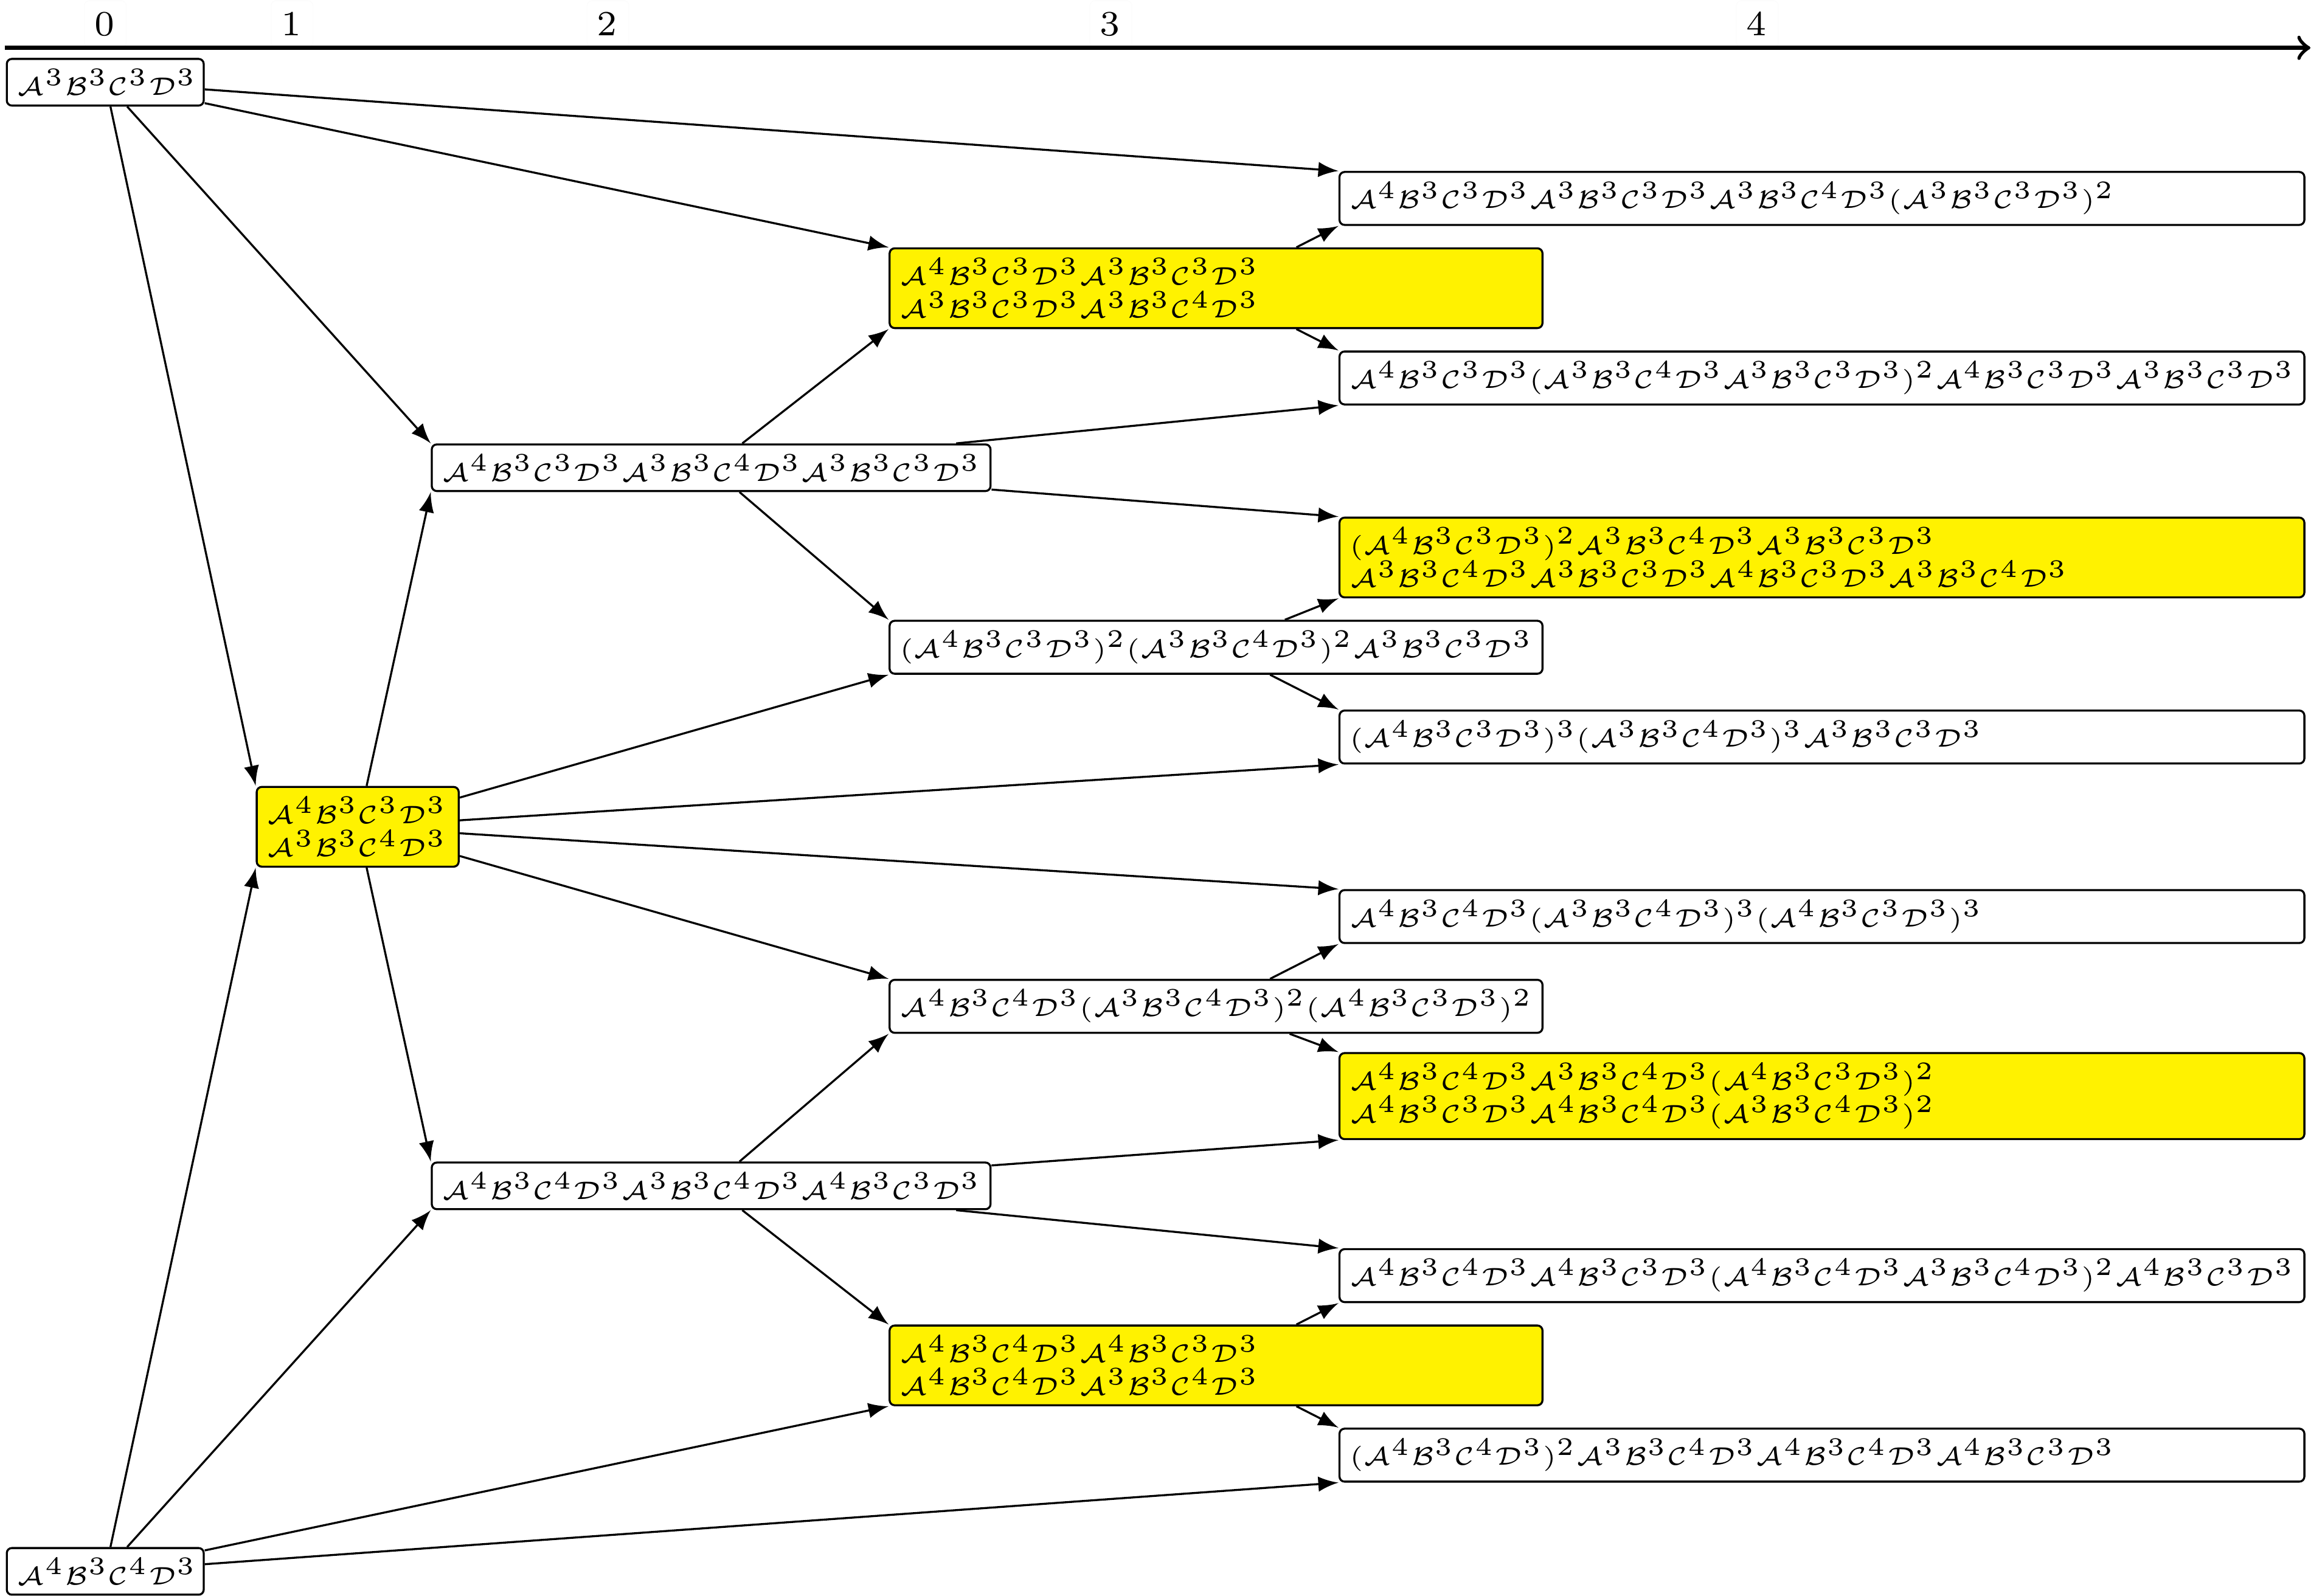
\includegraphics[width=.7 \textwidth]{../Figures/7/7.21/adding.png}
	\caption[Farey-tree with the symbolic sequences of a horizontal \glsentrylong{pal} structure]{
		Farey-tree with the symbolic sequences associated with the parameter regions of the horizontal \gls{pal} structure marked with a red arrow in \Cref{fig:add.add.halved.hor} up to three levels.
		Nodes of parameter regions associated with two coexisting cycles are colored yellow.
	}
	\label{fig:add.prop.hor.tree}
\end{figure}

\begin{theorem}[Coexistence in Child Nodes]
	\label{theorem:child.coexistence}
	\begin{enumerate}
		\item The child of two nodes that are both associated with a single cycle each is associated with two coexisting cycles.
		\item The child of a node that is associated with a single cycle and a node that is associated with two coexisting cycles is associated with a single cycle.
		\item The child of two nodes that are both associated with two coexisting cycles each is associated with two coexisting cycles.
	\end{enumerate}
\end{theorem}

\begin{proof} \phantom{x}
	\begin{enumerate}
		\item A node that is associated with a single cycle in the archetypal model is the manifestation of a cycle with an odd number of rotations in the halved archetypal model.
		      The child of two nodes that are associated with cycles with an odd number of rotations in the halved archetypal model is associated with a cycle with an even number of rotations.
		      Therefore, this cycle then manifests as two coexisting cycles in the archetypal model.
		\item Analogously, the child node of one node that is associated with a cycle with an odd number of rotations and one node that is associated with a cycle with an even number of rotations is associated with a cycle with an odd number of rotations.
		      Therefore, this cycle then manifests as a single cycle in the archetypal model.
		\item And the child node of two nodes that are both associated with a cycle with an even number of rotations is associated with a cycle with an odd number of rotations.
		      Therefore, this cycle then manifests as two coexisting cycles in the archetypal model.
		      \hfill $\blacksquare$ % todo: next line? only if it fits on the same page tho
	\end{enumerate}
\end{proof}

This explains the pattern we can observe in the periods of the \gls{pal} structures in \Cref{sec:add.add.like}.
We take another look at the 1D period scan of the horizontal \gls{pal} structure between the parameter regions $P^{14}_3$ and $\left[P^{14}_3  \mid P^{12}_3\right]$ in \Cref{fig:add.add.like.hor.1D}.
We get the information, whether a parameter region in the structure was associated with two coexisting cycles from the Farey-tree in \Cref{fig:add.prop.hor.tree}.
The parameter region associated with the period $14$ is not associated with coexisting cycles, therefore the corresponding cycle in the halved archetypal model has an odd number of revolutions and its period is twice as high as the period associated with the same parameter region in the halved archetypal model, which is $7$.
The parameter region associated with the period $13$ is associated with coexisting cycles, therefore the corresponding cycle in the halved archetypal model has an even number of revolutions its period is the same as the period associated with the same parameter region in the halved archetypal mode.
The parameter region in between those two parameter regions is associated with the period $7 + 13 = 20$ in the halved archetypal model.
Also, its cycle has an odd number of revolutions, since it is the concatenation of one cycle with an even and one cycle with an odd number of revolutions.
We know from \Cref{theorem:period.pal} that this parameter region is associated with the period $40$ in the archetypal model.
This is true as we can observer this in the 1D period scan in \Cref{fig:add.add.like.hor.1D}.
Also, we know from \Cref{theorem:child.coexistence} that this parameter region is associated with two coexisting cycles.
This is true as we can see in the Farey-tree in \Cref{fig:add.prop.hor.tree}.

The third case of \Cref{theorem:child.coexistence} cannot be seen in the farey tree.
It is actually not possible in the \gls{pal} structures we are investigating here.
We will prove this next.

\begin{theorem}[No Coexistence in both Parent Nodes]
	\label{theorem:no.parent.coex}
	In the \gls{pal} structures we are investigating, no node has two parent nodes that are \textbf{both} associated with two coexisting cycles each.
\end{theorem}

\begin{proof} \phantom{x} \\
	The Farey-trees can be constructed in the following way.
	We write down both starting nodes in a list.
	Then, for each iteration we combine every pair of neighboring nodes according to the rules.
	The result is inserted between the two nodes that are combined.
	And the nodes created at each iteration are the nodes of the next level.

	We will now construct a Farey-tree where the content of the nodes is just whether the node is associated with coexistence, $c$, or not, $n$.
	The rules for combining nodes are from \Cref{theorem:child.coexistence}.
	We reformulate the statement in \Cref{theorem:no.parent.coex} to a concrete statement about the lists at each iteration.

	In all lists, there will be no neighboring nodes that both have the content $c$.
	This implies no two nodes that both have the content $c$ are combined to have a child node.
	So no node has two parent nodes that are both associated with two coexisting cycles.
	We will now prove this using induction.

	\begin{itemize}
		\item[n = 0] The starting nodes are both associated with two coexisting cycles, so the initial list is $\{n, n\}$.
			We can see, there are no two nodes with both content $c$ next to each other. \checkmark
		\item[n + 1] We assume that the current list of $2^n$ nodes has no two nodes with both content $c$ next to each other.
			We take a look at each possible pair of neighboring nodes.
			\begin{itemize}
				\item $\{\dots, n, n, \dots\}:$ We combine both nodes with content $n$, the resulting node has content $c$.
				      The resulting list is the list $\{\dots, n, c, n, \dots\}$.
				      This rule will therefore never cause two neighboring nodes to both have the content $c$.
				\item $\{\dots, n, c, \dots\}:$ We combine the node with content $n$ with the node with content $c$, the resulting node has content $n$.
				      The resulting list is the list $\{\dots, n, n, c, \dots\}$.
				      This rule will therefore also never cause two neighboring nodes to both have the content $c$.
				\item $\{\dots, c, n, \dots\}:$ We combine the node with content $c$ with the node with content $n$, the resulting node has content $n$.
				      The resulting list is the list $\{\dots, c, n, n, \dots\}$.
				      This rule will therefore also never cause two neighboring nodes to both have the content $c$.
			\end{itemize}
	\end{itemize}
	\hfill $\blacksquare$
\end{proof}
